\PassOptionsToPackage{round,authoryear}{natbib}
\PassOptionsToPackage{table,dvipsnames}{xcolor}
\documentclass[]{style/company_light} % switch to style/company_border for border variant
% Compile: bash build.sh, or use pdfLaTeX with BibTeX on Overleaf.

\usepackage[utf8]{inputenc}
\usepackage{hyperref}
\usepackage{url}
\usepackage{booktabs}
\usepackage{amsfonts}
\usepackage{amsmath}
\usepackage{nicefrac}
\usepackage{microtype}
\usepackage{graphicx}
\usepackage{subcaption}
\usepackage{multirow}
\usepackage{enumerate}
\usepackage{enumitem}
\usepackage[most]{tcolorbox}
\usepackage{adjustbox}
\usepackage{array}
\usepackage{amssymb}
\usepackage{float}
% Keep pdfLaTeX builds portable across TeX distributions whose sans-serif
% fonts do not expose expansion metrics to microtype.
\microtypesetup{expansion=false}
\setlength{\emergencystretch}{1.5em}

\newcommand{\yes}{\textcolor{ForestGreen}{$\checkmark$}}
\newcommand{\no}{\textcolor{red}{$\times$}}
\newcommand{\partialyes}{\textcolor{orange}{$\checkmark$}}
\NewDocumentCommand{\todo}
{ mO{} }{\textcolor{magenta}{\textsuperscript{\textit{TODO}}\textsf{\textbf{\small[#1]}}}}

% ── Placeholder marker ────────────────────────────────────────────────────────
% \ph{...} marks a value that is NOT measured. Rendered in magenta and
% underlined so it cannot be mistaken for a real result, on screen or in print.
% Every occurrence must be replaced or removed before submission.
\newcommand{\ph}[1]{\textcolor{magenta}{\underline{\textsf{#1}}}}

% Custom commands from original paper
\newcommand\mc[1]{\mathcal{#1}}
\newcommand{\mbf}[1]{\mathbf{#1}}

% ── Metadata ──────────────────────────────────────────────────────────────────

% Global names for the paper's benchmark and method.  Change these two
% definitions to rename the system consistently across the manuscript.
\newcommand{\BenchmarkName}{Quant-Arena}
\newcommand{\MethodName}{RSI-Quant}

% Canonical display names for backbone models used in the experiments.
\newcommand{\ModelClaudeOpus}{Claude~Opus~5}
\newcommand{\ModelClaudeSonnet}{Claude~Sonnet~4.6}
\newcommand{\ModelDeepSeek}{DeepSeek~V4~Flash}
\newcommand{\ModelGemini}{Gemini~3.1~Pro}
\newcommand{\ModelGPTSol}{GPT-5.6-Sol}
\newcommand{\ModelGrok}{Grok~4.6}
\newcommand{\ModelKimi}{Kimi~K3}


\title{Quant-Arena: Benchmarking LLM Agents for Budgeted Quantitative Research}

\author{Navers Lab, Einsia.AI}
% TODO: replace with the real author list, e.g.
% \author[1,\dag]{Given Family}
% \affiliation[1]{Navers Lab, Einsia.AI}
% \contribution[\dag]{Equal contribution.}

\abstract{%
Quantitative research is an iterative loop: a researcher proposes a market hypothesis, implements it as an executable signal, tests it on historical data, and decides what to keep. Existing benchmarks score formulas, code, or individual trading decisions, leaving open whether large language models (LLMs) can complete this loop and produce strategies that work beyond the research period. We introduce \textbf{\BenchmarkName}, a benchmark and public leaderboard for end-to-end quantitative research on real A-share market data. A model constructs features and stock-scoring code, receives feedback only on 2022--2023, and freezes one strategy for assessment on the sealed year 2024. A cash-account evaluator applies trading constraints and costs, including market impact estimated from a simulated order book. Scores combine signal quality, excess return, token efficiency, and the diversity of features used by the strategy. We evaluate six frontier models in one-shot and iterative settings. Iteration raises 2024 returns for five of the six models. No one-shot strategy beats the equal-weight market, whereas the best iterative strategy (\ModelClaudeOpus) earns 13.3 percentage points of excess return. In a two-model feedback ablation, withholding performance metrics while retaining execution errors lowers mean 2024 returns for both models. Higher predictive correlation can still accompany lower portfolio returns, and all evaluated models trail Kepler-1, our closed-source professional strategy. \BenchmarkName\ is open to submissions from any model or agent harness.
}


\date{\today}
\metadata[HomePage]{\url{https://lab.einsia.ai/naversquant}}

% ── Document ──────────────────────────────────────────────────────────────────

\begin{document}

\maketitle

\section{Introduction}

Quantitative trading seeks to turn noisy market observations into signals and portfolios that generate reliable out-of-sample returns. Formulaic alphas provide an executable and interpretable representation of such signals \citep{Kakushadze2016Formulaic}. A quantitative research workflow repeatedly formulates a market hypothesis, translates it into a computational strategy, evaluates the resulting signal, and uses the outcome to choose what to test next. Financial data are noisy and non-stationary, the candidate space is large, and only a fraction of hypotheses remain useful beyond the observations that motivated them. Large language models (LLMs) can support this workflow through hypothesis generation, code synthesis, and analysis of experimental feedback. Recent alpha-discovery methods illustrate the growing range of research procedures built around these capabilities \citep{Wang2023AlphaGPT,Tang2025AlphaAgent,Han2026QuantaAlpha}.

Evaluating an LLM research agent introduces three closely related challenges. First, a final strategy reflects both the underlying model and the harness that organizes its prompts, tools, memory, candidate revisions, and stopping decisions. Comparisons therefore require a clearly specified unit of evaluation. Second, historical market data support repeated adaptive experimentation, creating opportunities for selection bias and backtest overfitting \citep{Bailey2017Backtest}. The research feedback available to an agent must be separated from the evidence used to judge its frozen output. Third, operational choices affect the outcome: unequal model budgets, different data access, silent retries, and inconsistent return conventions can change the apparent ranking of otherwise comparable systems. A benchmark must make these choices part of the evaluation contract.

These challenges motivate a system-level question: how effectively can an LLM agent use a fixed research budget to produce predictive signals and cost-adjusted research returns under a fixed historical protocol? Answering this question requires observing the research process, including unsuccessful attempts, resource consumption, and final selection. It also requires precise financial semantics. A cross-sectional signal statistic, a fixed-notional research return, and a funded account outcome measure different properties of a strategy. Their interpretation depends on the information cutoff, holding period, missing data, and costs. In particular, annualizing the mean of a few observable cohorts does not establish performance over a fully observed calendar interval.

We introduce \textbf{\BenchmarkName}, a benchmark and execution platform for budgeted quantitative research on real historical market data. A participant consists of a registered language model and a research harness. The harness proposes executable stock-scoring strategies, receives authorized research feedback, and commits one final strategy per replicate for sealed assessment. One-shot generation, ordinary feedback iteration, and external harnesses can therefore be compared as explicit research procedures. Section~\ref{sec:benchmark} defines the suite that holds their evaluation conditions fixed.

The Arena platform makes the research process inspectable across service boundaries. Strategy programs access market observations through date-scoped authorization, while trusted services retain model credentials, evaluate outputs, and settle resource usage. Durable operation records allow recoverable interruptions to resume accepted work without silently generating a new model response. A shared financial core connects internal factor research and Arena assessment, with access and disclosure policies specific to each setting.

The daily benchmark developed here uses raw-price observations for a registered Shenzhen A-share population. It fixes a signal--entry--exit alignment, Top-$K$ selection with complete boundary ties, half-notional overlapping cohorts, and an explicit cost convention. Financial outcomes are accompanied by coverage, predictive statistics, and resource observations with completeness flags. Metric availability and ranking eligibility are reported separately. The current diversity gate can return zero when quality evidence is missing; its feature-level reasons are therefore essential to interpretation. This paper describes the protocol and platform implementation. Campaign results are left open.

The contributions of this work are:
\begin{itemize}
    \item \textbf{A benchmark for budgeted research episodes.} We define the model--harness pair as the participant and evaluate its research and selection process, retaining unsuccessful attempts and resource records.
    \item \textbf{An explicit financial evaluation protocol.} We formalize temporal alignment, portfolio selection, research returns, missing observations, and score qualification, with separate evidence for simulated account behavior.
    \item \textbf{An Arena execution platform.} We implement controlled market-data access, isolated strategy execution, durable budget accounting, final strategy commitment, and recoverable evaluation, together with campaign records for reproducible comparison.
\end{itemize}

\section{\BenchmarkName: Task and Evaluation Protocol}
\label{sec:benchmark}

\BenchmarkName\ evaluates a complete quantitative research run, from the first model interaction to a frozen strategy's sealed assessment. The benchmark specifies the comparison contract; the Arena platform executes that contract. This separation allows research procedures to vary while preserving the information and measurement rules used to judge their outputs.

\subsection{Task, Participant, and Evaluation Unit}
\label{sec:arena_task}

We define a benchmark suite as
\begin{equation}
    q = (\mathcal{D},\mathcal{U},\mathcal{W},\mathcal{P},\mathcal{E},\mathbf{B},\mathcal{F},\mathcal{V}),
    \label{eq:arena_task}
\end{equation}
where $\mathcal{D}$ identifies immutable data releases, $\mathcal{U}$ the authorized instrument population, $\mathcal{W}$ the chronological windows and warmup rules, $\mathcal{P}$ the input profile, $\mathcal{E}$ the execution environment, $\mathbf{B}$ the resource budgets, $\mathcal{F}$ the feedback policy, and $\mathcal{V}$ the financial and scoring evaluator. All components are frozen before a matched comparison. A change to this contract defines a new benchmark setting.

A participant $a=(M,H)$ combines a registered language model $M$ with a research harness $H$. The harness determines prompt construction, candidate generation, feedback interpretation, stopping, and final selection. A replicate executes this participant under $q$ with a registered seed identifier and its own budget. An episode contains the prescribed replicates; their complete records constitute the unit of comparison. Harness changes, including different prior memories or candidate-selection policies, define participant variants under the same suite.

The platform supports three input profiles: authorized raw market data, fifteen-second order-book observations, and anonymous numerical features. They expose different information and preprocessing requirements and are evaluated as distinct conditions. Strategies return cross-sectional stock scores for authorized signal dates and may declare constituent features. Optional training uses an earlier registered interval; the resulting model artifact is frozen and reused in research and final evaluation. Both participant-defined scoring programs and trusted linear combinations of declared features are supported. The latter provide directly verifiable feature-use evidence for diversity assessment.

\subsection{Research Interaction and Resource Constraints}
\label{sec:arena_interaction}

The harness alternates between model interactions and admitted research evaluations. Each completed evaluation returns the projection permitted by $\mathcal{F}$, including selected metrics, validity and coverage information, execution summaries, and remaining resources. Metric precision and available diagnostics are fixed by the suite. Private signal matrices, quantitative execution logs, fitted artifacts, and trading records are withheld from the research feedback channel.

The current budget profile distinguishes model tokens, admitted research evaluations, and execution CPU usage. Let $u_j$ be the reported token usage of model operation $j$, $n_{\mathrm{adm}}$ the number of admitted research evaluations, and $c_\ell$ the measured CPU usage of execution $\ell$. The corresponding usage vector is
\begin{equation}
    \mathbf{b} = \left(\sum_j u_j,\ n_{\mathrm{adm}},\ \sum_\ell c_\ell\right),
    \qquad \mathbf{b} \preceq \mathbf{B}
    \quad\text{for budget-eligible runs}.
    \label{eq:budgets}
\end{equation}
These sums apply when the required usage records are known; unresolved usage retains an explicit unavailable state. Admission also accounts for outstanding reservations and protects CPU capacity for final evaluation. Reservations are released or settled against observations and do not become measured consumption by definition. CPU accounting covers registered executions rather than all shared-service overhead. Token ceilings do not imply equal monetary expenditure or equal effective computation across models.

A malformed model reply consumes its observed tokens. A strategy rejected before evaluation admission does not consume an admitted evaluation; an accepted evaluation retains its evaluation charge if execution subsequently fails. Data requests and bytes remain metered under the current service-limit profile, with access and concurrency controls; historical profiles retain their own cumulative resource definitions.

Three participation modes establish different research conditions. \emph{One-shot} returns one complete strategy and freezes it, without research feedback, model-assisted repair, or additional training; platform documents may be read on request, and those reads are charged as ordinary model calls. \emph{Vanilla} uses a model--feedback conversation: the model may finish with a completed candidate, and the last completed candidate with feedback is the declared fallback when the budget ends. \emph{External harnesses} implement their own search and selection rules through the same authorized services. Their external knowledge, memory initialization, repair policy, and selection rule form part of the participant specification.

\subsection{Temporal Access and Final Commitment}
\label{sec:arena_contract}

Training, research, and final accounting windows are registered chronologically. Authorized warmup supplies historical context without extending the accounting interval. For a signal date $d$, the executable strategy receives only observations in the authorized data release, instrument and field scope, and availability interval ending at $\kappa(d)$. The cutoff $\kappa(d)$ is registered with the suite and is not disclosed in the public contract. Data permissions are enforced by the execution service rather than inferred from dates supplied by participant code.

After research, each replicate commits one strategy. Its source, runtime, fitted artifact when present, and declared feature configuration are fixed before sealed assessment. The harness controls the selection; the platform validates and freezes the commitment and runs the final evaluator. Final-window outcomes are excluded from candidate revision within that replicate. Further evaluation under another contract produces a separate record and preserves the original result.

The daily protocol uses registered static Shenzhen A-share factor columns. Missing observations are retained, and no daily index-constituent mask is imposed. Population construction, delisted securities, and data-publication history must therefore be disclosed alongside the suite. Runtime authorization controls access during the experiment; historical knowledge in model pretraining or participant priors remains a separate source of possible contamination. Repeated public leaderboard access also requires a campaign-level disclosure policy, as discussed in Appendix~\ref{app:boundary}.

\subsection{Daily Financial Evaluation}
\label{sec:arena_returns}
% DRAFT (Claude, factual skeleton): prose to be rewritten by Gemini; keep the
% wording rules: "bought on T, sold on T+1 with an algorithmic order"; slippage
% "computed from order-book limits and market impact, not a fixed value".

Index consecutive trading sessions by $t$. Scores $s_{i,t-1}$ are formed using information authorized through session $t-1$. A selected cohort is bought on trading day $t$ and sold on day $t+1$ with an algorithmic order. Slippage is computed from order-book limits and market impact; it is not a fixed value. Limit-up stocks are not bought, halted or limit-down positions are sold once they become tradable, and no replacement stocks are selected. An authorized predecessor signal can support the first entry day; an absent predecessor is not reconstructed from later data, and missing source rows produce no signal.

\paragraph{Selection.}
Let $\mathcal{I}_t$ contain the registered instruments with finite scores for entry $t$, ranked in descending order. For a valid signal row, let $s_{[k],t-1}$ be its $k$-th largest score and define
\begin{equation}
    k_t=\min(K,|\mathcal{I}_t|),\qquad
    \mathcal{S}^{K}_t=\{i\in\mathcal{I}_t:s_{i,t-1}\ge s_{[k_t],t-1}\}.
    \label{eq:topk}
\end{equation}
This definition includes every boundary tie, so the selected count may exceed $K$. Selection precedes the observation of forward prices and does not replace securities whose returns later prove unavailable. The primary basket uses $K=75$; $K\in\{200,400\}$ are retained as diagnostics.

\paragraph{Research returns.}
Let $y_{i,t}$ be the realized raw-price return of stock $i$ over the cohort's holding period and $\mathcal{A}^{K}_t\subseteq\mathcal{S}^{K}_t$ the selected stocks with a valid return. The cohort research return $r^K_t$ is the equal-weight mean of $y_{i,t}$ over $\mathcal{A}^K_t$, net of trading costs. Cohorts overlap and returns accumulate additively:
\begin{align}
    R^K &= \sum_{t\in\mathcal{J}_K}r^K_t,
    &\operatorname{ARR}^{K} &= \frac{243}{|\mathcal{J}_K|}\sum_{t\in\mathcal{J}_K}r^K_t,\label{eq:research_arr}\\
    \Delta\operatorname{ARR}^{K} &= \frac{243}{|\mathcal{J}^{\cap}_K|}
       \sum_{t\in\mathcal{J}^{\cap}_K}(r^K_t-r^{\mathrm{mkt}}_t),
       \label{eq:excess_arr}
\end{align}
where $\mathcal{J}_K$ are entry sessions with an available return, $r^{\mathrm{mkt}}_t$ is the full-market Shenzhen A-share reference under the same convention, and $\mathcal{J}^{\cap}_K$ are paired sessions. An empty observable set yields an unavailable return rather than zero. Signed additive drawdown is
\begin{equation}
    \operatorname{DD}^{K}
    =\min_{0\le j\le |\mathcal{J}_K|}
       \left(P^K_j-\max_{0\le h\le j}P^K_h\right)\le0,
    \label{eq:drawdown}
\end{equation}
with $P^K_j$ the cumulative sum through the $j$-th available cohort. The long-only Sharpe ratio is $\mathrm{SR}_L=\sqrt{243}\,\overline{r^{75}}/\operatorname{sd}(r^{75})$. The long--short Sharpe ratio $\mathrm{SR}_{LS}$ applies the same annualization to the daily raw return of the top score decile minus the bottom decile; it measures the signal's discriminative power, not a tradable return. Because adjacent cohorts overlap, both ratios are descriptive. A funded cash account is simulated and reported separately from research returns.

\subsection{Scoring}
\label{sec:scoring}
\label{sec:arena_scoring}
% DRAFT (Claude): formulas are final; prose to be rewritten by Gemini.

On each valid entry date, RankIC is the cross-sectional rank correlation between $s_{i,t-1}$ and $y_{i,t}$; $\overline{\mathrm{RankIC}}$ is its daily mean and RankICIR the mean divided by the sample standard deviation. Turnover $\mathrm{TO}\in[0,1]$ is the mean daily fraction of the Top75 basket that is replaced. With $x^+=\max(0,x)$, the in-sample (2022--2023) quality score is the weighted geometric mean
\begin{equation}
    Q=\Big(\sqrt{\overline{\mathrm{RankIC}}^{+}}\Big)^{w_1}
      \Big(\tfrac{A^+}{1+A^+}\Big)^{w_2}
      \Big(\tfrac{\mathrm{SR}_L^+}{1+\mathrm{SR}_L^+}\Big)^{w_3}
      \Big(\tfrac{\mathrm{SR}_{LS}^+}{1+\mathrm{SR}_{LS}^+}\Big)^{w_4}
      \Big(\tfrac{1}{1+\mathrm{TO}}\Big)^{w_5},
    \qquad A=\mathrm{RankICIR}\cdot\sqrt{243},
    \label{eq:quality}
\end{equation}
with $(w_1,\dots,w_5)=(0.225,0.225,0.225,0.225,0.1)$. Each term lies in $[0,1]$ with diminishing returns. Turnover enters as $1/(1+\mathrm{TO})$ so that a fully rotating basket halves this term instead of zeroing $Q$. Efficiency and diversity are
\begin{equation}
    E=Q\left(1-\frac{T}{B}\right),\qquad
    D=Q\,\frac{\min(K,32)}{32},
    \label{eq:efficiency}
\end{equation}
where $T$ is the provider-reported token usage, $B=500{,}000$ the token budget, and $K$ the number of qualified, used, and mutually independent feature clusters (Appendix~\ref{app:diversity}). The window score is
\begin{equation}
    S=\begin{cases}70Q+20E+10D & \text{one-shot and vanilla tracks},\\ 80Q+20D & \text{system and custom tracks,}\end{cases}
    \label{eq:overall}
\end{equation}
on a 0--100 scale, and the leaderboard total is
\begin{equation}
    \mathrm{Total}=0.3\,S_{\mathrm{in}}+0.7\,S_{\mathrm{out}}.
    \label{eq:total}
\end{equation}
The in-sample formula, its parameters, and all component scores are published. The out-of-sample (2024) score $S_{\mathrm{out}}$ takes into account RankIC, IC stability, long-only and long--short Sharpe ratios, turnover, factor diversity, and token usage; its combination is not disclosed and may be revised independently. Raw metrics of both windows are published.

Unavailable metrics retain reason codes and sample counts and are never replaced by zero. Failed runs remain in every denominator; averages over completed runs only are labelled as conditional statistics.

\section{Arena Execution and Reproducibility}
\label{sec:arena}

The Arena platform implements the benchmark contract across participant interaction, market-data access, strategy execution, and final scoring. Its control plane records suites, submissions, replicates, operations, resource usage, and results. Quantitative workers and data services execute the authorized computation. A batch campaign interface uses these same services to compare declared combinations of models, harnesses, budgets, and suites.

\subsection{Separation of Research and Quantitative Execution}
\label{sec:arena_execution}

The research harness controls what to propose and when to evaluate or finish. It receives model and research tools, while computational strategies execute under a separate identity with scoped market-data access. A trusted evaluator consumes the resulting scores and applies the frozen financial rules. This division allows an agent to conduct data-intensive research through executable programs without forwarding raw market matrices or private evaluation artifacts into the model conversation. Table~\ref{tab:arena_roles} summarizes the responsibilities.

\begin{table}[t]
    \centering
    \small
    \caption{Responsibilities within the Arena. The final choice belongs to the participant; execution permissions, accounting, and assessment belong to the platform.}
    \label{tab:arena_roles}
    \begin{tabular}{@{}p{0.20\linewidth}p{0.35\linewidth}p{0.36\linewidth}@{}}
        \toprule
        Component & Controlled decisions & Recorded or returned evidence \\
        \midrule
        Research harness & Prompts, candidate revisions, stopping, final selection & Model interactions, research actions, selected strategy \\
        Strategy execution & Computation within the authorized input and runtime contract & Daily scores, declared features, optional fitted artifact \\
        Model gateway & Model access, operation identity, usage settlement & Provider response, observed usage, unresolved-operation state \\
        Data and execution services & Version binding, date and field scope, process lifecycle & Authorized execution records, resource observations \\
        Trusted evaluator & Labels, trading rules, metrics, qualification & Core results, coverage, private detailed evidence \\
        Campaign interface & Registered comparison matrix and collection & Existing scorecards, complete replicate and failure registry \\
        \bottomrule
    \end{tabular}
\end{table}

Model-provider credentials and data-access capabilities are held by trusted services. In the reusable execution environment, a supervisor advances the frozen sequence of signal dates. Each date starts a fresh low-privilege strategy process, working directory, and date-scoped data gateway. Before advancing, the supervisor closes the day's processes and connections and persists its accepted output. Reusing the virtual machine therefore preserves controlled execution infrastructure; participant state crosses stages only through declared artifacts such as a frozen fitted model. Earlier per-day runtime contracts remain identifiable by their registered versions.

Training, research, and final assessment use separately bound executions. The final evaluator accepts registered sealed releases through a private data plane, while research credentials retain their authorized research scope. The resulting boundary combines service authorization with process isolation. Claims about a hosted campaign additionally depend on the deployed runtime, network configuration, and boundary checks recorded for that campaign.

\subsection{Immutable Data and Shared Financial Evaluation}
\label{sec:arena_data}

Market observations are served from immutable publications. Offline preparation establishes the data layout, indexes, calendar, and declared coverage. Online access resolves the authorized release and reads bounded dates, instruments, and fields. Daily data use published queryable stores; indexed intraday data support column and time-range selection. Exact price and quantity semantics, exchange-local timestamps, and source missingness are retained through the query interface. A change to the default publication does not redirect an active suite away from its registered version.

Arena and the internal research platform use a shared daily replay and statistical core. Within one daily evaluation, market observations support forward labels, the full-market reference, research cohorts, and cash accounts under the same conventions. This limits semantic drift between financial research and benchmark reporting. Access and disclosure policies remain specific to each setting: a research interface's visible-date cutoff alone does not establish a sealed evaluation release. Likewise, common evaluation code supports consistency, while agreement of deployed entry points requires matched end-to-end run evidence.

The three input profiles are bound to actual releases before use. Raw-event processing, fifteen-second observations, and anonymous features introduce different preprocessing and information conditions; platform support alone does not establish that a dataset has been publicly released or used in a completed campaign. Publication receipts and coverage summaries identify the data underlying each leaderboard setting.

\subsection{Durable Accounting and Recoverable Progress}
\label{sec:arena_recovery}

Model calls, strategy registration, research evaluations, and final commitments carry persistent operation identities. The platform records budget reservations separately from observed consumption. Provider-reported counters settle model usage, and trusted execution measurements settle CPU usage when available. Unreported usage remains unknown. This separation keeps conservative admission estimates from appearing as measured costs.

A harness can checkpoint and yield while an evaluation runs, then resume from its saved research state. Strategy execution persists accepted daily outputs so that recoverable interruptions can continue the remaining dates. Completed model operations are recovered under their original identities. When a request's provider outcome or charge cannot be established, the operation remains unresolved pending reconciliation; it is not automatically replaced by another generation. Recovery thus preserves the candidate history and resource boundary of the original replicate.

The evaluator persists core financial and signal results before optional reference comparisons, reports, and detailed artifact publication. A failure in an optional step affects that evidence and any dependent component, while preserving the core result. Participant errors, infrastructure blockage, cancellation, and statistical unavailability remain distinct outcomes. These are properties of the execution design; campaign completion rates, recovery success, and runtime overhead are empirical quantities to be reported separately.

\subsection{Campaigns and Reproducibility Records}
\label{sec:arena_campaigns}

The campaign interface snapshots the declared participant source and public suite contract, persists submission intent, and submits through the shared Arena services. It collects evaluator-produced scorecards without recomputing financial results. Direct comparisons bind the service origin, suite, selected runtime, budget definition, and protocol. Different input scopes or financial conventions define separate groups.

A reproducibility record links the data publication, suite, participant source and prior information, actual model identity, model interactions, admitted trials, usage observations, final commitment, and final scorecard. All prescribed replicates remain visible in the campaign record, including failed, cancelled, blocked, and incomplete runs. Stored model replies support reconstruction of an observed trajectory; new calls to an external provider need not reproduce that trajectory exactly. The registration requirements appear in Appendix~\ref{app:registry}.

\section{RSI Harness}
\label{sec:harness}

% Pending: leave this section empty until the implementation is available.
% Define RSI, state and updates, tools and priors, generation and repair,
% budget allocation, stopping and final selection, version and freeze point.

\section{Experiments}
\label{sec:experiments}

\subsection{Experimental Setup}
\label{sec:setup}

We evaluate \ModelClaudeOpus, \ModelAstra, \ModelDeepSeek, \ModelGemini, \ModelGLM, and \ModelKimi\ using the platform's standard research harness. Models develop strategies on the 2022--2023 research period, and their frozen programs are assessed on the sealed year 2024. Each independent research attempt has a budget of 500,000 model tokens.

We compare two research settings. \textbf{One-shot} asks the model to produce a complete strategy without research-performance feedback. The harness permits corrections to invalid proposals. \textbf{Iterative research} allows the model to revise candidates using return, signal-quality, coverage, and execution-error feedback, with at most five candidate evaluations. The model then commits one completed strategy for assessment. Both settings use the data access and financial evaluation defined in Section~\ref{sec:benchmark}.

The main comparison follows the leaderboard selection: for each model and setting, we report the retained entry with the highest overall score among eligible submissions. Existing retained entries are used when scores tie. Each row contains the scores and financial metrics of that same strategy. Individual submissions remain available for the supplementary analysis. We include our closed-source strategy Kelper-1 as a professional reference and compare returns against the equal-weight market reference over the same assessment period. The market reference is gross of trading costs.

We report the overall score, research-period and assessment-period scores, and the assessment-period annualized return (ARR), excess ARR, long-only Sharpe ratio, and maximum drawdown (MDD). Excess ARR is the difference from the market reference, expressed in percentage points. The errors-only control described in Section~\ref{sec:feedback_effect} uses the same research budget and evaluation rules while withholding performance feedback.

\subsection{Overall Performance}
\label{sec:main}

% Keep the main results and their NAV curves together on the page.
\begin{table*}[!t]
    \begin{minipage}{\linewidth}
        \begin{table}[H]
  \caption{Main comparison under the \BenchmarkName\ contract. Every arm uses the same markets, seeds, proposal budget, expression language, factor-fusion model, portfolio simulator, and confirmation evaluator. Factor predictive power and strategy performance are reported separately, with validity and token usage retained as search diagnostics. Values are placeholders pending the final frozen campaigns; the released version will additionally report each market--seed cell.}
  \label{tab:main}
  \centering
  \small
  \begin{tabular}{lrrrrrrr}
    \toprule
    Arm & \multicolumn{2}{c}{\textbf{Factor Predictive Power}} & \multicolumn{3}{c}{\textbf{Strategy Performance}} & \multicolumn{2}{c}{\textbf{Search Diagnostics}} \\
    \cmidrule(lr){2-3} \cmidrule(lr){4-6} \cmidrule(lr){7-8}
    & Rank ICIR & ICIR & IR (SHR*) & ARR (\%) & MDD (\%)$\downarrow$ & Valid (\%) & Tokens \\
    \midrule
    B0: native benchmark                & \ph{TBD} & \ph{TBD} & \ph{TBD} & \ph{TBD} & \ph{TBD} & \ph{TBD} & \ph{TBD} \\
    H0: fixed stateful harness          & \ph{TBD} & \ph{TBD} & \ph{TBD} & \ph{TBD} & \ph{TBD} & \ph{TBD} & \ph{TBD} \\
    H1: prompt evolution                & \ph{TBD} & \ph{TBD} & \ph{TBD} & \ph{TBD} & \ph{TBD} & \ph{TBD} & \ph{TBD} \\
    H2: retrieval/planning evolution    & \ph{TBD} & \ph{TBD} & \ph{TBD} & \ph{TBD} & \ph{TBD} & \ph{TBD} & \ph{TBD} \\
    V2: YAML capability study           & \ph{TBD} & \ph{TBD} & \ph{TBD} & \ph{TBD} & \ph{TBD} & \ph{TBD} & \ph{TBD} \\
    V3: source capability study         & \ph{TBD} & \ph{TBD} & \ph{TBD} & \ph{TBD} & \ph{TBD} & \ph{TBD} & \ph{TBD} \\
    \bottomrule
  \end{tabular}
\end{table}

    \end{minipage}
    \par\vspace{1em}
    \begin{minipage}{\linewidth}
        \captionsetup{type=figure}
        \centering
        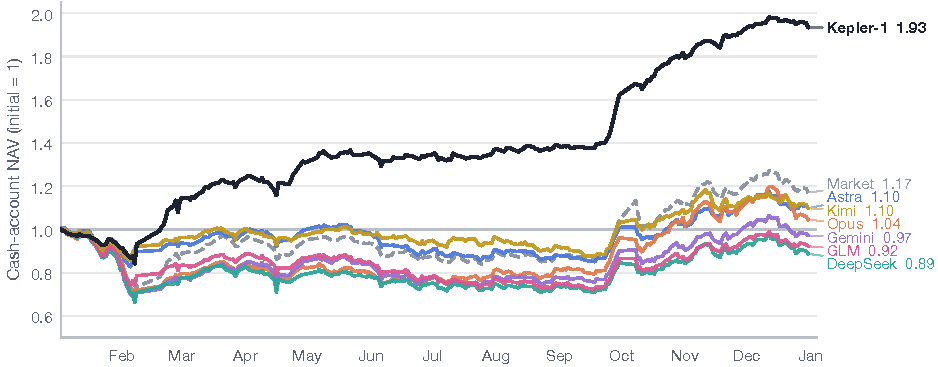
\includegraphics[width=\linewidth]{Figures/fig_nav.pdf}
        \caption{Out-of-sample cash-account NAV in 2024 for the six selected iterative strategies in Table~\ref{tab:main}, our closed-source reference Kelper-1, and the equal-weight market reference. All series use initial capital of 1. The market reference is gross of trading costs.}
        \label{fig:nav}
    \end{minipage}
\end{table*}

The highest-scoring model entry in Table~\ref{tab:main} is Opus with iterative research, at 31.9 points, followed by Astra at 30.3 and DeepSeek at 29.5. All remain below the professional reference, which scores 52.5. The separation is also visible in returns: Opus achieves 30.4\% ARR, compared with 88.3\% for Kelper-1.

Positive returns do not consistently translate into outperformance. Four of the six selected iterative strategies have positive ARR, but only Opus and DeepSeek exceed the market reference, by 13.3 and 1.9 percentage points, respectively. Astra earns 16.4\% and Kimi 9.8\%, both below the reference. Gemini and GLM lose money despite receiving research feedback. Among the five models with retained entries in both settings, all one-shot strategies underperform the market.

Research-period scores and assessment-period outcomes also differ. Astra has the highest research-period score among models, at 36.7, but ranks behind Opus and DeepSeek on the sealed period. Gemini's score falls from 24.6 to 4.0, while GLM's falls from 13.5 to 0.0. Risk adds another distinction: DeepSeek's selected strategy has a Sharpe ratio of 1.16 and a maximum drawdown of 7.9\%, compared with 0.92 and 31.1\% for Opus. The higher-return strategy therefore does not dominate on risk.

Figure~\ref{fig:nav} shows the corresponding cash-account NAV paths throughout 2024.

\subsection{Effects of Research Feedback}
\label{sec:feedback_effect}
\label{sec:e2}

Iterative research improves the selected overall score for all five models with results in both settings. Excess ARR improves for four, with gains ranging from 7.5 percentage points for GLM to 39.0 for DeepSeek. Gemini is the exception: its score rises from 0.0 to 10.2, but its excess ARR falls by 4.3 percentage points.

To examine the role of performance feedback, we compare full feedback with an \textbf{errors-only} control for Astra and DeepSeek. Both conditions use the same research budget and evaluation rules. The control withholds performance metrics and score-derived labels while retaining execution status, errors, candidate identifiers, and remaining-budget information. Models can still repair their code, revise strategies, and select a completed candidate. Table~\ref{tab:feedback} compares the retained control entries with the full-feedback entries in Section~\ref{sec:main}.

\begin{table*}[t]
\centering
\footnotesize
\caption{Full performance feedback versus errors-only feedback. Each row reports one selected iterative strategy. ARR, excess ARR, and RankIC refer to 2024. Tokens are total model tokens consumed during research, in thousands. The selected Astra control is one of three completed controls tied at an overall score of zero.}
\label{tab:feedback}
\setlength{\tabcolsep}{6pt}
\begin{tabular}{@{}llrrrrr@{}}
\toprule
Model & Feedback & Overall & ARR (\%) & Excess (pp) & RankIC & Tokens (k) \\
\midrule
\ModelAstra & Full & 30.3 & 16.4 & $-0.7$ & 0.0462 & 95.7 \\
 & Errors only & 0.0 & $-6.5$ & $-23.5$ & 0.0018 & 50.3 \\
\midrule
\ModelDeepSeek & Full & 29.5 & 18.9 & +1.9 & 0.0494 & 418.2 \\
 & Errors only & 0.0 & $-3.1$ & $-20.2$ & $-0.0044$ & 155.1 \\
\bottomrule
\end{tabular}
\end{table*}


Both selected errors-only strategies score zero. Full-feedback entries achieve higher excess ARR by 22.9 percentage points for Astra and 22.0 for DeepSeek, alongside RankIC values of 0.0462 and 0.0494 rather than values near zero. The other two completed Astra controls also have negative excess returns.

The selected full-feedback attempts also use more of the available research budget. Astra evaluates four candidates instead of one, and DeepSeek five instead of three, with higher token consumption in both cases. These comparisons measure feedback-driven research under a common budget, including the additional computation used during revision.

\subsection{Predictive Signal versus Portfolio Outcome}
\label{sec:signal_vs_portfolio}

Strong signal statistics do not guarantee a strong portfolio. In the iterative track, all five models reach similar 2024 RankIC (0.029--0.049), yet their 2024 excess returns span 38 percentage points, from $+13.3$ to $-24.9$. The two models with the \emph{highest} in-sample RankIC, \ModelGemini\ (0.064) and \ModelGLM\ (0.056), produce the \emph{worst} 2024 portfolios. Their long--short Sharpe ratios fall to zero or below. \ModelClaudeOpus\ has the lowest 2024 RankIC of the five (0.029) but the best portfolio and a long--short Sharpe of 1.51.

RankIC measures how well a strategy orders the whole market. The portfolio depends only on the top 75 stocks, and on whether they can actually be bought and held under price limits. A model that optimizes average correlation can improve the ordering of thousands of uninteresting stocks while leaving the head of the ranking no better than chance. This is why \BenchmarkName\ scores signal and portfolio terms jointly, and why the geometric mean in Equation~\eqref{eq:quality} requires every term to be positive.

\subsection{Effect of Reasoning Effort}
\label{sec:effort}

\begin{figure}[t]
    \centering
    \figorph{Figures/fig_effort.pdf}{\linewidth}{Reasoning effort}
    \caption{Effect of reasoning effort. Total score and tokens used for each model at each reasoning setting. \ph{Results pending.}}
    \label{fig:effort}
\end{figure}

Reasoning effort is the main inference-time setting that participants control. For each model whose provider exposes a working control, we run both tracks at a low and a high setting, in addition to the default, under the same suite and budget. Providers control reasoning in different ways: discrete effort levels, explicit thinking budgets, or an on/off switch. Some models cannot vary it at all. We use each provider's native control and report the reasoning tokens actually consumed.

\phtext{Results pending: per-model findings on whether more reasoning improves the committed strategy, how it changes token use and therefore $E$, and whether it helps one-shot more than iterative research.}

\subsection{What Happens During Research}
\label{sec:process}

We compare the first executable candidate of each completed iterative run with the strategy it finally commits to. Eight of nine runs improve their in-sample excess return over that trajectory, by 10.6 percentage points on average. No run commits to its first candidate, and six commit to the candidate with the best in-sample result. Models therefore use feedback actively and select greedily on the research window. Because only the committed strategy is assessed on 2024, this improvement is in-sample progress. Section~\ref{sec:main} shows that it transfers unevenly.

\begin{figure}[t]
    \centering
    \figorph{Figures/fig_tokens_vs_score.pdf}{\linewidth}{Tokens vs score}
    \caption{Tokens used versus total score for all completed runs. Official runs are highlighted.}
    \label{fig:tokens}
\end{figure}

Token use and score are only loosely related (Figure~\ref{fig:tokens}). \ModelAstra\ reaches 30.29 with 96k tokens, while \ModelGemini\ and \ModelGLM\ spend about 370k tokens for scores of 10.22 and 4.05. \ModelClaudeOpus\ and \ModelDeepSeek\ spend 320k and 418k for the top two out-of-sample scores. Spending more of the budget helps only when the model can turn feedback into better candidates.

\subsection{Reliability}
\label{sec:reliability}

\begin{table}[t]
\centering
\small
\caption{Run outcomes per model and track in the main campaign (snapshot of 18 October 2026). Attempts exclude runs cancelled by the operators because of platform or model-provider incidents, and runs still in progress. A completed run has a frozen strategy with a sealed assessment.}
\label{tab:attempts}
\begin{tabular}{@{}lrrrrrr@{}}
\toprule
 & \multicolumn{3}{c}{One-shot} & \multicolumn{3}{c}{Iterative} \\
\cmidrule(lr){2-4}\cmidrule(l){5-7}
Model & Att. & Done & Failed & Att. & Done & Failed \\
\midrule
\ModelClaudeOpus & 10 & 3 & 7 & 3 & 2 & 1 \\
\ModelAstra & 3 & 3 & 0 & 3 & 3 & 0 \\
\ModelDeepSeek & 3 & 3 & 0 & 1 & 1 & 0 \\
\ModelGemini & 4 & 3 & 1 & 2 & 2 & 0 \\
\ModelGLM & 3 & 1 & 2 & 1 & 1 & 0 \\
\ModelKimi & 7 & 2 & 5 & 1 & 0 & 1 \\
\bottomrule
\end{tabular}
\end{table}


Completing a research run is itself a capability. Table~\ref{tab:attempts} reports all attempts in the main campaign, excluding runs cancelled because of platform or provider incidents. Failure rates differ sharply by model. Here a failure means the run produced no valid committed strategy: an invalid proposal, a strategy that fails during execution, or a harness protocol failure.
\begin{itemize}[leftmargin=*,itemsep=1pt]
    \item \ModelAstra\ and \ModelDeepSeek\ completed every attempt.
    \item \ModelClaudeOpus\ failed 7 of 10 one-shot attempts.
    \item \ModelKimi\ failed 5 of 7 one-shot attempts and its only iterative attempt.
\end{itemize}
\ModelKimi's failures occurred through a third-party relay and its runs through the official API are pending. \ph{Failure breakdown by cause pending.} A model that cannot reliably produce an executable strategy in one pass has a lower expected score in practice than its best run suggests.

\phtext{Stability across repeated runs of the same model and track is analyzed separately.}

\section{Related Work}
\label{sec:related}

\subsection{Formulaic Alpha Mining with Language Models}

Formulaic alpha mining searches for executable expressions that transform market observations into predictive cross-sectional signals. Published formula libraries demonstrate the interpretability and executability of this representation \citep{Kakushadze2016Formulaic}. Automated approaches then use evolutionary search or learned generators to explore expression spaces and combine the resulting factors \citep{Zhang2020AutoAlpha,Shi2024AlphaForge}. These explicit search spaces support reproducible execution, but they are combinatorial, highly exposed to noisy backtest feedback, and often optimized around a narrow factor statistic rather than the behavior of the final portfolio.

LLMs extend this paradigm by connecting economic hypotheses, symbolic construction, and empirical diagnosis. LLMFactor uses sequential knowledge-guided prompting to extract interpretable factors from financial information \citep{Wang2024LLMFactor}; Automate Strategy Finding with LLM combines multimodal market inputs with a multi-agent portfolio workflow \citep{Kou2024AutomateStrategy}; Alpha-GPT introduces interactive LLM-based alpha generation \citep{Wang2023AlphaGPT}; AlphaAgent regularizes generation for originality, hypothesis--factor alignment, and structural simplicity \citep{Tang2025AlphaAgent}; and QuantaAlpha treats a complete mining trajectory as the unit of evolution and reuses effective sub-trajectories through mutation and crossover \citep{Han2026QuantaAlpha}. These systems establish the value of structured, multi-stage alpha discovery beyond one-shot formula generation. \BenchmarkName\ provides a common contract for evaluating such research procedures as model--harness participants, with executable strategy outputs, explicit resource use, and a frozen final-assessment boundary.

\subsection{Self-Improving Agents and Recursive Search}

Memory and iterative feedback are central to self-improving LLM agents. General agent frameworks such as ReAct interleave reasoning with environment actions \citep{Yao2023ReAct}, while Reflexion and Self-Refine use textual feedback and iterative revision without changing model parameters \citep{Shinn2023Reflexion,Madaan2023SelfRefine}. Voyager demonstrates how an executable skill library can support open-ended, lifelong improvement \citep{Wang2023Voyager}. In finance, FinMem organizes market information with layered memory for trading decisions \citep{Yu2023FinMem}, QuantAgent couples an inner response-refinement loop with an outer knowledge-base update loop \citep{Wang2024QuantAgent}, FactorMiner retains successful patterns, failure constraints, and reusable skills \citep{Wang2026FactorMiner}, and QuantaAlpha preserves trajectory-level evidence for evolutionary refinement \citep{Han2026QuantaAlpha}. AQuA closes bounded loops in which validated experimental evidence guides subsequent proposals, whereas QuantEvolver converts quantitative evaluation into policy-update signals through reinforcement fine-tuning \citep{Guo2026AQuA,Zhang2026QuantEvolver}. Together, these approaches show that improvement can occur through memory retrieval, structured candidate evolution, recursive experimentation, or model-parameter updates.

\BenchmarkName\ treats these forms of adaptation as participant properties. Within-run memory and search policy belong to the registered harness; across-run learning additionally requires a declared development history and a frozen evaluation variant. The benchmark fixes the data boundary, resource definitions, feedback, and financial evaluator so that different adaptive procedures can be compared under stated conditions.

\subsection{Quantitative Benchmarks and Evaluation Protocols}

Existing financial infrastructure serves several different evaluation goals. Qlib standardizes AI-oriented quantitative workflows, while FinRL provides reinforcement-learning environments and trading evaluations \citep{Yang2020Qlib,Liu2020FinRL}. Financial language benchmarks such as FinBen and Finance Agent Benchmark evaluate domain understanding, generation, forecasting, and research tasks \citep{Xie2024FinBen,Bigeard2025FinanceAgent}. General agent benchmarks such as AgentBench and MLAgentBench examine multi-turn interaction, tool use, and iterative experimentation \citep{Liu2023AgentBench,Huang2023MLAgentBench}. AlphaBench focuses on formulaic alpha generation, evaluation, and search \citep{Luo2026AlphaBench}, and recent trading-agent evaluation also examines leakage, attribution, and memory effects \citep{Zhu2026KTDFin}.

AlphaForgeBench is a close comparison: it treats LLMs as quantitative researchers that generate executable factors and strategies, separating model reasoning from backtest execution \citep{Zhang2026AlphaForgeBench}. Its published evaluation uses standardized prompts, independent code generations, and a common backtest engine. Executable outputs and the separation of reasoning from execution are therefore shared design choices. Table~\ref{tab:benchmark_scope} contrasts the documented comparison procedures.

\begin{table}[t]
    \centering
    \footnotesize
    \caption{Protocol scope relative to AlphaForgeBench \citep{Zhang2026AlphaForgeBench}, based on its published pipeline and experimental settings (Sections 3.2 and E.3, version 2). ``Not specified'' describes these passages and does not establish that a capability is absent from its software.}
    \label{tab:benchmark_scope}
    \begin{tabular}{@{}>{\raggedright\arraybackslash}p{0.18\linewidth}>{\raggedright\arraybackslash}p{0.34\linewidth}>{\raggedright\arraybackslash}p{0.40\linewidth}@{}}
        \toprule
        Dimension & AlphaForgeBench & \BenchmarkName \\
        \midrule
        Comparison unit & Independent generations per query and model & Model--harness episodes with prescribed replicates \\
        Research procedure & Standardized prompts and generation settings & Registered harnesses with explicit search and selection policies \\
        Resource boundary & Fixed generation count; cumulative search ledger not specified & Per-replicate admission, reservations, charges, and observed usage \\
        Feedback and selection & Generate-and-backtest pipeline & Authorized research feedback followed by one frozen final strategy \\
        Final assessment & Common historical backtest & Separately authorized sealed final interval \\
        Failure and recovery & API failure disclosed; operation recovery and unknown usage not specified & Failed attempts retained; unresolved operations and measurements explicit \\
        Financial basis & Single-asset strategy backtests across assets & Cross-sectional research cohorts and separate funded accounts \\
        \bottomrule
    \end{tabular}
\end{table}


Our focus is the resource-bounded process that selects a final strategy. Repeated backtest feedback introduces selection bias \citep{Bailey2017Backtest}, while interrupted execution can change the effective search budget if retries generate unrecorded candidates. \BenchmarkName\ makes the model--harness pair, feedback boundary, final commitment, failed attempts, and unresolved measurements part of the evaluation record. Arena recovery preserves operation identity and accepted progress under those rules. These mechanisms define the intended comparison scope; their effect on rankings, completion, and cost requires campaign evidence.

\section{Conclusion}
\label{sec:conclusion}

We introduced \BenchmarkName, a benchmark and open leaderboard that evaluates LLMs on complete quantitative research runs. A model researches with bounded feedback on 2022--2023 data, commits one strategy, and is assessed once on a sealed 2024 window. The assessment uses a cash account with realistic execution constraints, and the score covers signal quality, excess return, efficiency, and feature diversity.

Our first evaluation of six frontier models gives three findings.
\begin{itemize}[leftmargin=*,itemsep=1pt]
    \item Performance feedback is what makes LLM research work. Without it, no model beats the market; with it, the best model earns 13.3 percentage points of excess return.
    \item In-sample progress and predictive correlation are poor proxies for out-of-sample portfolio value. Models with the strongest research-window signals produced some of the weakest 2024 portfolios.
    \item All models remain far below a professional reference strategy.
\end{itemize}
\BenchmarkName\ is open to submissions from any model or agent harness. We plan to add markets, input profiles such as order-book data and anonymized features, and fresh sealed windows.


% ── Contributions ────────────────────────────────────────────────────────────

\clearpage
\newpage

\definecolor{brandcolor}{RGB}{227, 170, 121}
\section{Contributions and Acknowledgements} The contributors' names are sorted in alphabetical order of the last name.

\textbf{Project Lead}

% TODO

\textbf{Core Contributors}

% TODO

\textbf{Contributors}

% TODO

\textbf{Team Management}

% TODO

\textbf{Corresponding to} % TODO

\textbf{Acknowledgements.} This project is founded and supported by Navers Lab, Einsia.AI.

% ── References ──────────────────────────────────────────────────────────────

\clearpage
\newpage
\bibliographystyle{assets/plainnat}
\bibliography{ref}

% ── Appendix ─────────────────────────────────────────────────────────────────

\clearpage
\newpage
\appendix

\section{Suite Registry and Reproducibility}
\label{app:registry}

A suite supplies the concrete values underlying Equation~\eqref{eq:arena_task}. This revision describes the current daily research protocol, identified as \texttt{sandbox\_daily\_research\_v2}, from implementation revision \texttt{7889d4f}. These identifiers locate the implementation basis of the description; the deployed campaign revision and its actual data releases must be registered independently. Historical suites retain their original result, runtime, and budget conventions.

Table~\ref{tab:suite_registry} lists the campaign-specific fields to complete before reporting results. The financial conventions in Table~\ref{tab:daily_protocol} do not determine data size, sample dates, model identity, or resource ceilings. No values for those fields are inferred from implementation defaults.

\begin{table}[ht]
    \centering
    \small
    \caption{Campaign registration fields. The value column is intentionally blank until actual suite and run records are available.}
    \label{tab:suite_registry}
    \begin{tabular}{@{}p{0.23\linewidth}p{0.57\linewidth}p{0.12\linewidth}@{}}
        \toprule
        Field & Required specification & Value \\
        \midrule
        Data release & Provider, market, release identity, provenance, access and publication scope &  \\
        Data coverage & Dates, securities, event counts, fields, missingness and its denominator &  \\
        Population & Static column construction, inclusion rules, delistings, reference population &  \\
        Temporal windows & Training, research, final, warmup, cutoff, label realization &  \\
        Sealed history & Release identity, sealing time, prior availability and exposure policy &  \\
        Participants & Model/provider identity, parameters, harness source, prompts, prior memory &  \\
        Resources & Per-replicate ceilings; final reserve; observed versus charged usage; token and CPU completeness &  \\
        Runtime & Selected image, execution protocol, data-service and evaluator revision &  \\
        Replicates & Prescribed identifiers, seed handling, statuses, frozen selection references &  \\
        Scores & Calibration, weights, risk and statistical thresholds, reference bank and policy &  \\
        Comparison & Primary endpoint, financial/composite eligibility, coverage strata, evidence minimum and tie policy & \\
        Reporting & Aggregation, uncertainty, failure policy, result release and retained artifacts &  \\
        \bottomrule
    \end{tabular}
\end{table}

\paragraph{Research and model records.}
Each run retains its model interactions and observed usage, candidate registrations, admitted evaluations, feedback, operation outcomes, and final-selection record. A source snapshot identifies the harness that generated the sequence. External information and preinitialized memory are part of the participant declaration. Provider-returned model identities and usage counters supplement configured display names. Unknown counters and uncertain paid operations remain explicit.

\paragraph{Financial and execution records.}
The final commitment binds strategy source, runtime, fitted artifact, and feature configuration. The corresponding evaluation retains the frozen dates and data releases, accepted daily execution records, core metrics, coverage, and private detailed evidence. Optional artifact failures retain their own status. Public scorecards expose authorized summaries; private trading records and data-sensitive artifacts follow the registered access policy.

\paragraph{Aggregation and release.}
Each campaign lists every prescribed replicate, including incomplete and unsuccessful ones. Complete aggregates require all corresponding values, with metric sample counts preserved. Financial eligibility, general eligibility, composite availability, and paper-specific coverage strata remain separate recorded fields. Each table row links to its episode and evaluator-owned final scorecards; token and CPU completeness accompany observed usage. Publication changes the authorized visibility of saved results; it does not redefine their financial convention. Imported or locally declared reference results retain their evidence status and are separated from evaluator-verified Arena results. Stored responses permit reconstruction of the observed research sequence, without assuming a future provider call is deterministic.

\section{Information Boundary and Qualification Rules}
\label{app:boundary}

\subsection{Authorization and Final-Assessment Boundary}

The research harness receives its public suite, authorized tools, research feedback, and remaining-resource state. Quantitative strategy execution receives a separately scoped market-data capability. The trusted supervisor holds that capability and mediates requests through the permitted version, dates, instruments, fields, and availability cutoff. Participant programs cannot expand the scope by supplying another date or forwarding their own internal authorization headers. Final evaluation uses the registered sealed release through the private data plane.

A final commitment ends candidate selection for that replicate. The same frozen strategy and trained artifact, when present, are used for sealed assessment. Recovery continues the recorded operation and accepted progress; it does not authorize a new candidate or new paid model response. A separate replay or changed evaluation contract creates a separate result and preserves the original commitment.

This boundary addresses runtime access and evaluation ownership. It does not establish that historical information was absent from a model's training data or a participant's prior resources. Organizers must document population construction, earlier publication of data, development experiments, and the method freeze point. Public leaderboard feedback can also influence later submissions. Campaign registration therefore specifies the intended experiment set and disclosure policy, retaining all attempts used for the reported comparison. Periodically refreshed or separately retained final windows are possible governance extensions, rather than assumed properties of the current runtime.

\subsection{Exact Diversity Construction}
\label{app:diversity}

Diversity is computed only when actual feature use can be verified. Feature directions and the reference bank are frozen with the strategy and suite. A feature must satisfy registered observation and coverage requirements, exceed its predictive-quality threshold, and have a positive one-sided lower confidence bound under the registered moving-block bootstrap. The confidence calculation adjusts for the number of declared feature comparisons. Bootstrap block length, resamples, seed, quality basis, and thresholds are suite parameters. This gate provides statistical qualification under those parameters; it does not establish a distinct economic mechanism.

For two features $f$ and $g$, let $\mathcal{T}_{fg}$ be dates with sufficient paired observations and nonconstant ranks. Subject to the registered overlap and sample conditions, their similarity is
\begin{equation}
    \sigma(f,g)=\frac{1}{|\mathcal{T}_{fg}|}
       \sum_{t\in\mathcal{T}_{fg}}
       \left|\operatorname{Corr}\!\left(
          \operatorname{rank}(f_t),\operatorname{rank}(g_t)\right)\right|.
    \label{eq:feature_similarity}
\end{equation}
Ranks are computed on each date's paired observations with average ranks for ties. For the current daily profile, overlap coverage compares paired finite coordinates with the finite union inside the authorized universe; coordinates absent from both features do not count as disagreement. An insufficient comparison is unavailable, rather than zero similarity.

Let $\mathcal{G}$ be the qualified, consumed feature set. Form an undirected graph with one vertex per feature and an edge when $\sigma(f,g)\ge\tau$, where $\tau$ is registered in advance. Let $C(\mathcal{G})$ be its number of connected components. For feature $f$, let $\mathcal{R}_f$ be the comparable members of the frozen reference bank. When the required pairwise and reference comparisons are available, define
\begin{equation}
    \nu_f=1-\max_{r\in\mathcal{R}_f}\sigma(f,r),\qquad
    D=\frac{\min\{C(\mathcal{G}),C_{\max}\}}{C_{\max}}
       \frac{1}{|\mathcal{G}|}\sum_{f\in\mathcal{G}}\nu_f.
    \label{eq:diversity}
\end{equation}
Thus, diversity rewards qualified groups and novelty relative to the declared bank. Graph components are correlation-based groups, without a claim of probabilistic independence.

The reference-comparison policy is frozen. The available-reference policy uses only comparisons that pass the unchanged sample conditions and reports the total reference count, comparable counts, and coverage. The historical all-required policy requires every registered reference to be comparable. Missing within-set comparisons or an empty required reference set leave $D$ unavailable. If the completed quality assessment finds no qualified feature, $D=0$; if quality cannot be assessed because the required evidence is missing, the result remains unavailable. Unverified feature use also leaves $D$ unavailable.

\subsection{Metric Availability and Ranking Eligibility}

Execution completion, strategy freezing, metric availability, and leaderboard eligibility are separate states. A finite research return can coexist with insufficient observations for IC, an unavailable full-market reference, or unverified feature use. Each metric retains its value or unavailability reason, relevant sample count, and coverage. Absence of optional evidence does not discard completed financial results.

Financial rankings apply their registered financial, resource, and risk requirements. They do not require unrelated IC or diversity evidence. The composite in Equation~\eqref{eq:overall} additionally requires its nonzero-weight components, calibration, and complete usage evidence. In particular, a default positive diversity weight makes unverified feature use incompatible with a complete composite, while financial results remain reportable. These qualification rules are fixed before observing final outcomes.

\paragraph{Verification evidence.}
Contract tests can check deterministic temporal alignment, denial of unauthorized observations, budget charging, final-commitment rules, and recovery behavior. Real-data agreement between research and Arena entry points additionally requires the same factor, dates, market release, parameters, runtime versions, and complete financial records. The existence of a shared evaluator or a passing synthetic test alone does not establish deployed agreement. Operational rates and runtime costs require actual campaign measurements.


\end{document}
